\section{Model mismatch: $k$-component graph}

\begin{figure}[!htb]
    \centering
    \begin{subfigure}[b]{0.3\textwidth}
        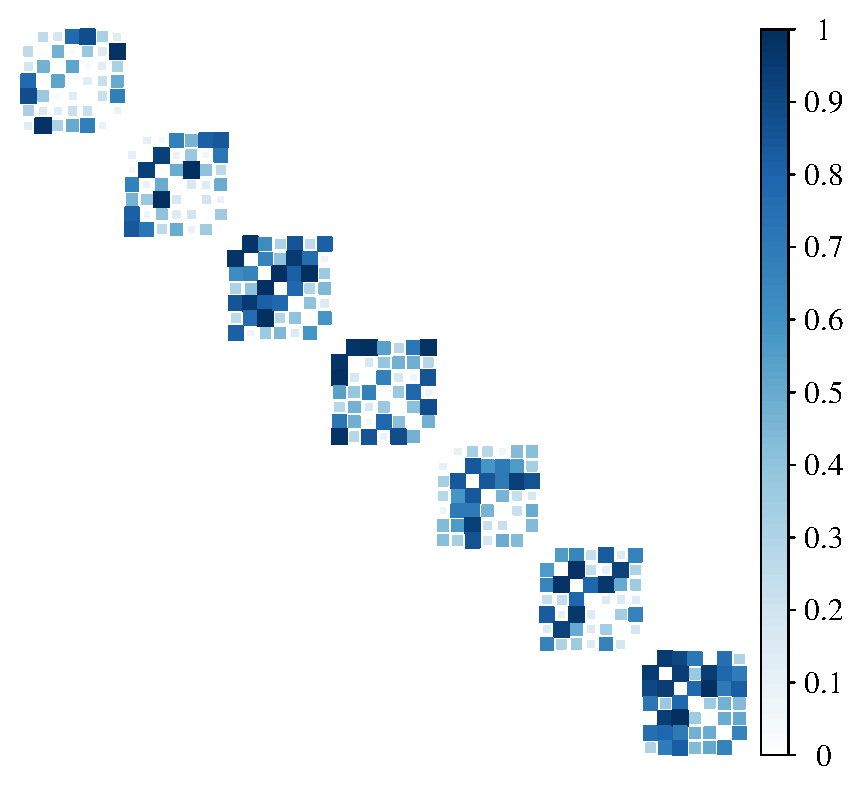
\includegraphics[width=\textwidth]{model-mismatch/true_mat.eps}
        \caption{Ground Truth Laplacian matrix}
    \end{subfigure}
    ~ %add desired spacing between images, e. g. ~, \quad, \qquad, \hfill etc.
      %(or a blank line to force the subfigure onto a new line)
    \begin{subfigure}[b]{0.3\textwidth}
        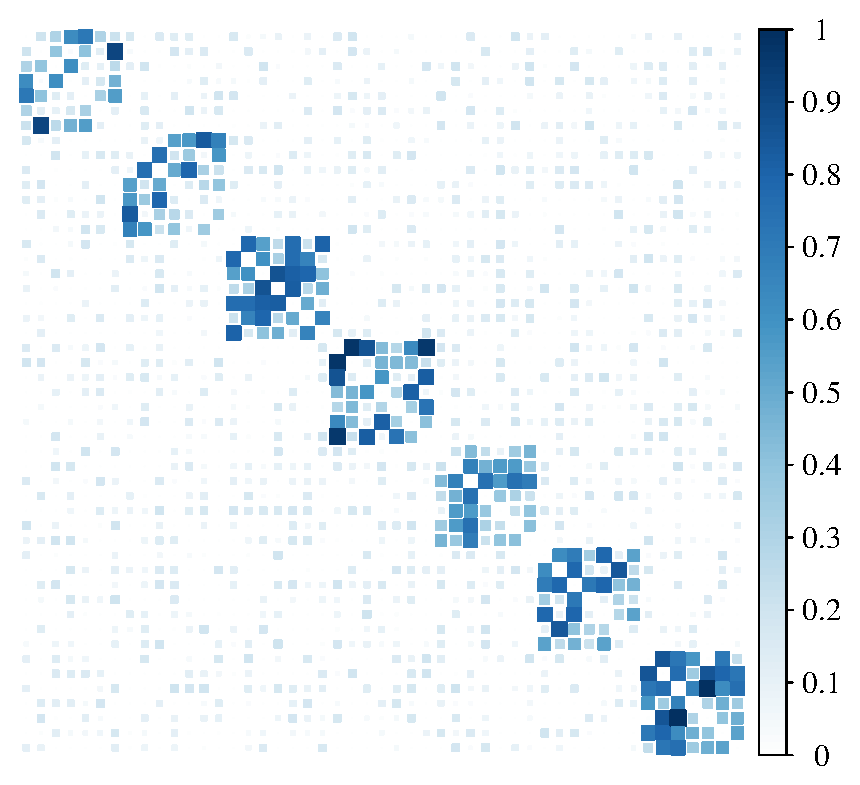
\includegraphics[width=\textwidth]{model-mismatch/noisy_mat.eps}
        \caption{Noisy Laplacian matrix}
    \end{subfigure}
    ~ %add desired spacing between images, e. g. ~, \quad, \qquad, \hfill etc.
    %(or a blank line to force the subfigure onto a new line)
    \begin{subfigure}[b]{0.3\textwidth}
        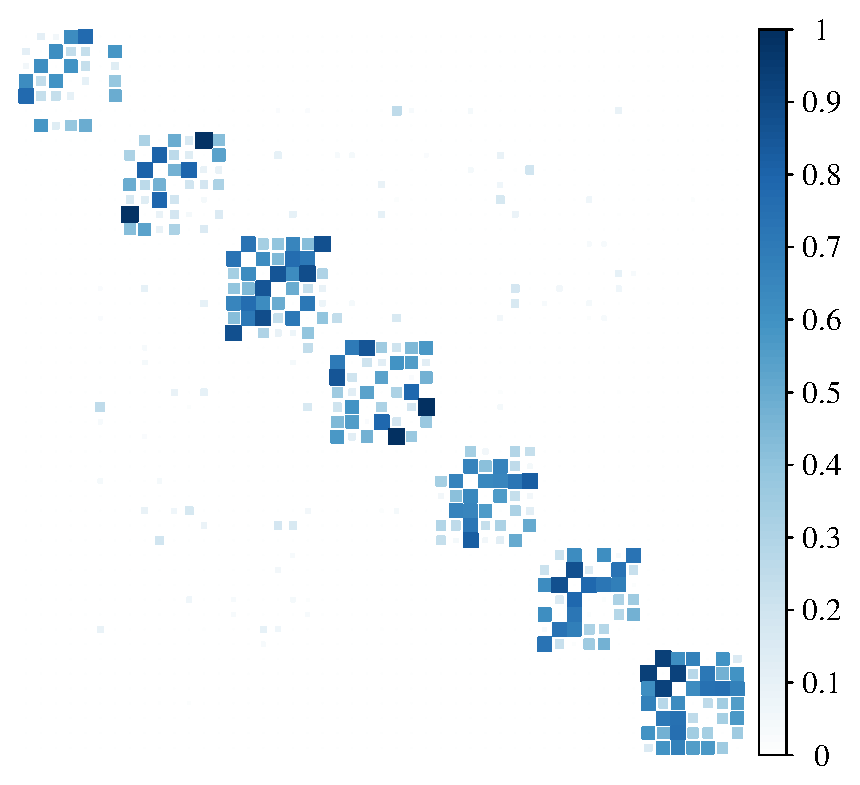
\includegraphics[width=\textwidth]{model-mismatch/est_mat.eps}
        \caption{Learned Laplacian matrix}
    \end{subfigure}
        \\
    \begin{subfigure}[b]{0.3\textwidth}
        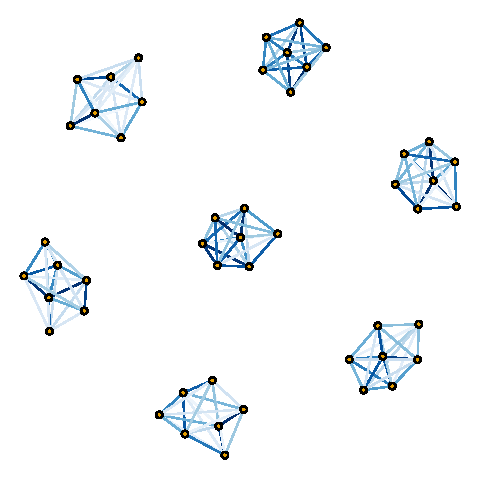
\includegraphics[width=\textwidth]{model-mismatch/true_graph.eps}
        \caption{Ground Truth graph}
    \end{subfigure}
    ~ %add desired spacing between images, e. g. ~, \quad, \qquad, \hfill etc.
      %(or a blank line to force the subfigure onto a new line)
    \begin{subfigure}[b]{0.3\textwidth}
        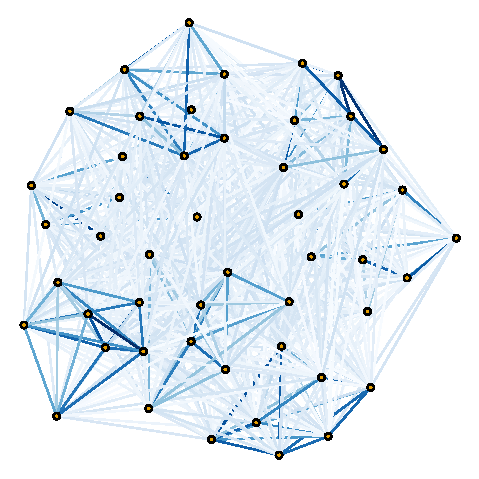
\includegraphics[width=\textwidth]{model-mismatch/noisy_graph.eps}
        \caption{Noisy graph}
    \end{subfigure}
    ~ %add desired spacing between images, e. g. ~, \quad, \qquad, \hfill etc.
    %(or a blank line to force the subfigure onto a new line)
    \begin{subfigure}[b]{0.3\textwidth}
        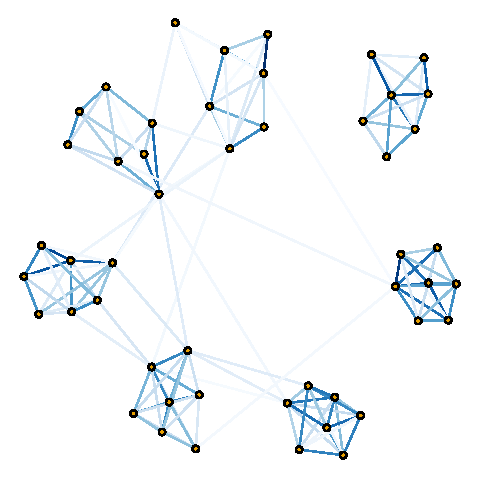
\includegraphics[width=\textwidth]{model-mismatch/est_graph.eps}
            \caption{Learned graph}
    \end{subfigure}
        \caption{An example of estimating a 4-component graph. (a) the ground truth graph Laplacian matrix ($\mathbf{L}_{\mathsf{true}}$),
                 (b) $\mathbf{L}_{\mathsf{true}}$ after being corrupted by noise, (c) the learned graph Laplacian with a performance of
                 $(\mathsf{RE}, \mathsf{FS}) = (0.210, 1)$.
                 The panels (d), (e), and (f) correspond to the graphs represented by the Laplacian matrices in
                 (a), (b), and (c), respectively.}\label{fig:4-comp-graph}
        \label{fig:4-comp}
\end{figure}
